% CVPR 2026 Paper Template

\documentclass[10pt,twocolumn,letterpaper]{article}

%%%%%%%%% PAPER TYPE  - PLEASE UPDATE FOR FINAL VERSION
% \usepackage{cvpr}              % To produce the CAMERA-READY version
\usepackage[review]{cvpr}      % To produce the REVIEW version
% \usepackage[pagenumbers]{cvpr} % To force page numbers, e.g. for an arXiv version

% Import additional packages in the preamble file, before hyperref
%% This file contains a number of tweaks that are typically applied to the main document.
%% They are not enabled by default, but can be enabled by uncommenting the relevant lines.

%%
%% Pins a figure to render exactly where it is declared in the source, rather
%% than letting LaTeX's float algorithm search ahead/behind for "the best" spot
%%
\usepackage{float}

%% Omit CreationDate/ModDate (and their time zone) from the PDF info dictionary.
\pdfinfoomitdate=1

%%
%% Inline annotations; for predefined colors, refer to "dvipsnames" in the xcolor package:
%% https://tinyurl.com/overleaf-colors
%%
\newcommand{\red}[1]{{\color{red}#1}}
\newcommand{\todo}[1]{{\color{red}#1}}
\newcommand{\TODO}[1]{\textbf{\color{red}[TODO: #1]}}
%%
%% disable for camera ready / submission by uncommenting these lines  
%%
% \renewcommand{\TODO}[1]{}
% \renewcommand{\todo}[1]{#1}

%%
%% work harder in optimizing text layout. Typically shrinks text by 1/6 of page, enable
%% it at the very end of the writing process, when you are just above the page limit
%%
% \usepackage{microtype}

%%
%% fine-tune paragraph spacing
%%
% \renewcommand{\paragraph}[1]{\vspace{.5em}\noindent\textbf{#1.}}

%%
%% globally adjusts space between figure and caption
%%
% \setlength{\abovecaptionskip}{.5em}


%%
%% Allows "the use of \paper to refer to the project name"
%% with automatic management of space at the end of the word
%%
% \usepackage{xspace}
% \newcommand{\paper}{ProjectName\xspace}

%%
%% Commonly used math definitions
%%
% \DeclareMathOperator*{\argmin}{arg\,min}
% \DeclareMathOperator*{\argmax}{arg\,max}

%%
%% Tigthen underline
%%
% \usepackage{soul}
% \setuldepth{foobar}

\definecolor{cvprblue}{rgb}{0.21,0.49,0.74}
\usepackage[pagebackref,breaklinks,colorlinks,allcolors=cvprblue]{hyperref}

%%%%%%%%% PAPER ID  - PLEASE UPDATE
\def\paperID{*****} % *** Enter the Paper ID here
\def\confName{CVPR}
\def\confYear{2026}

%%%%%%%%% TITLE
\title{Reinforcement-Learning-Scheduled Latent Diffusion for Visual Counterfactual Explanations, and What Ground-Truth-Anchored Evaluation Reveals About Them}

%%%%%%%%% AUTHORS
\author{Anonymous CVPR submission\\
Paper ID \paperID}

\begin{document}
\maketitle
\begin{abstract}
Visual counterfactual explanation methods for medical image classifiers are conventionally scored by Counterfactual Validity (CV): the rate at which a generated image flips the classifier's decision. We make two contributions that pull in opposite directions, and argue the second is the more consequential. First, we present PPO-CF, a system in which a PPO agent schedules the sampling procedure of a frozen, LoRA-adapted latent diffusion generator (selecting per-step noise strength, classifier- and preservation-guidance scales, refinement-pass count, guidance ramp-up point and stopping time) as an alternative to one hand-tuned schedule for every image, which may fit a heterogeneous population poorly; editing is largely confined to a dilated lung region by a soft, RePaint-style background lock. Second, we show that CV, computed as it usually is with the same classifier that guided generation, cannot by itself establish whether the edit is class-relevant. We introduce two measurements that do not share that circularity: a Lesion Hit Rate (LHR) anchored to radiologist-drawn opacity boxes, and a held-out transfer ratio that re-scores counterfactuals with classifiers that never participated in guidance. Under these, the picture changes substantially. On the RSNA Pneumonia Detection Challenge, our committed configuration attains a mean CV of 0.838 and a 2.67$\times$ LHR lift over the annotation-area null ($p = 4.2 \times 10^{-53}$), yet on the most independent validator held-out transfer for n$\to$p remains in the adversarial regime (0.046 n$\to$p, 0.186 p$\to$n, against a 0.15 threshold). A five-arm study of trained policies (one training run per arm) produces two negative results: an annealed sparsity reward fails at its own objective and costs lesion targeting ($d = 0.512$), and a Grad-CAM spatial constraint collapses the base task entirely ($d = 1.205$, CV $0.838 \to 0.017$). The committed ensemble-guided policy also targets lesions better than an earlier single-classifier policy (paired $d = 0.482$), but that policy predates our split and seeding controls (\S\ref{sec:controls}) and likely differs in other training settings as well, so the gain cannot be attributed to ensembling alone.
% TODO: "likely differs" rests on development history (reward weights, a1 range, anchoring), unverified for the trained arm
We argue that reporting CV without a ground-truth- or independence-anchored companion metric can substantially overstate progress, as it does for our own system.
\end{abstract}

\section{Introduction}
\label{sec:intro}

Classifiers deployed on chest radiographs are typically audited with attribution maps, which indicate where evidence is concentrated but not what change would alter the prediction. Visual counterfactual explanations close this gap: given a query image $x$ with prediction $f(x)$ and a target class $c$, a generator produces $x_c$ that (i) is scored at $c$ by the classifier, (ii) remains a realistic radiograph, and (iii) differs from $x$ only in a minimal, class-relevant region, preserving anatomy, foreign objects and patient identity.

Two observations motivate this work. The first is a modelling one. A fixed, hand-tuned guidance schedule may fit a heterogeneous test population poorly: if some images need only a gentle nudge across the decision boundary and others aggressive multi-pass editing, one schedule would either under-edit the latter or de-realize the former. We therefore frame per-step guidance control as a sequential decision problem and train a PPO agent to schedule it against a reward that trades classification progress against preservation and realism. The policy is conditioned on the image state and step index, so it can emit image- and step-dependent controls. The agent never touches the diffusion weights; it controls only the sampling procedure around a frozen generator, which keeps the action space small and the learned policy reusable at inference time on arbitrary query images.

The second observation is an evaluative one, and in retrospect the more important. The field's standard success criterion, Counterfactual Validity, is almost always computed with the same classifier whose gradients guided generation. It therefore cannot distinguish a genuine class-relevant edit from an adversarial perturbation tuned to one model. This is not a hypothetical concern in our setting: our own system reaches high CV while transferring poorly to classifiers that did not participate in guidance. We consider it a reporting problem for the subfield rather than a defect specific to our generator, and we address it with two companion measurements, one anchored to human annotation and one to model independence, which we recommend alongside CV.

\paragraph{Contributions.}
\begin{enumerate}
    \item PPO-CF: a PPO-scheduled sampling controller over a frozen, LoRA-adapted Stable Diffusion generator, with a soft, segmentation-gated background lock that blends the latent outside a dilated lung mask back toward the original image's latent at every denoising step (\S\ref{sec:method}).
    \item An evaluation protocol that pairs CV with a ground-truth-anchored Lesion Hit Rate and a held-out transfer ratio, together with the split-, seeding- and routing-level controls a control-arm comparison requires in order to mean anything (\S\ref{sec:evaluation}).
    \item A five-arm study of trained policies (one training run per arm), yielding two negative results (one of them the largest effect size we measure, against a mechanism designed to help) and one confounded improvement: the ensemble-guided policy beats an earlier single-classifier policy that differs from it in guidance and probably also in reward weights, $a_1$ range and anchoring (unverified; \S\ref{sec:controls}), so only a policy-free sweep bears on ensembling itself (\S\ref{sec:five-arms}--\ref{sec:negative-results}).
\end{enumerate}

\section{Related Work}
\label{sec:related}

\paragraph{Counterfactual explanation in medical imaging.} Singla \etal~\cite{singla2022explaining} introduced a GAN-based counterfactual generator for chest radiographs together with the evaluation protocol (Counterfactual Validity, FID, and Foreign-Object Preservation) that has become the de facto benchmark, and which we adopt for comparability. Their FOP metric depends on a Fast R-CNN foreign-object detector trained on private annotations, which is not reproducible offline; \S\ref{sec:conventional-metrics} describes our model-free substitute. Subsequent work has largely retained the same classifier-scored notion of validity~\cite{augustin2022diffusion,jeanneret2022diffusion,jeanneret2023adversarial}.

\paragraph{Diffusion-based counterfactuals.} Classifier- and gradient-guided diffusion sampling~\cite{dhariwal2021diffusion,meng2022sdedit,preechakul2022diffusion} has displaced GAN-based approaches for editable generation, owing to more stable training and higher sample fidelity. We build on a LoRA-adapted~\cite{hu2022lora} Stable Diffusion v1.5~\cite{rombach2022highresolution} backbone with DDIM sampling~\cite{song2021denoising} rather than training a diffusion model from scratch on a comparatively small radiograph corpus.

\paragraph{Spatially constrained editing.} RePaint~\cite{lugmayr2022repaint} and Blended Latent Diffusion~\cite{avrahami2022blended} re-noise and re-composite the unedited region at every denoising step. We adapt this as a soft background lock: rather than trusting the guidance gradient to keep edits inside the lung field, at every step the latent is blended, through a dilated, feathered lung mask, toward the original image's latent forward-diffused to the next timestep.

\paragraph{Localized counterfactuals.} ECED~\cite{luu2025visual} edits only a Score-CAM foreground; FiRe~\cite{zeng2026fire} adds saliency dual masks, adaptive guidance and early stopping; DocVCE~\cite{saifullah2025docvce} filters adversarial gradients. Our lock is mask-based, but a Grad-CAM mask collapsed our base task (\S\ref{sec:negative-results}); our schedule is learned around a frozen generator, not hand-designed. None reports LHR or held-out transfer or used our split and seeding; we do not compare head-to-head (Supp.~E3).

\paragraph{RL and diffusion.} Most RL work on diffusion fine-tunes the model weights against a reward (e.g.\ DDPO~\cite{black2024training}, reward-weighted fine-tuning). Treating the sampling hyperparameters as an RL action space around a frozen generator is comparatively unexplored, and is what we do here.

\section{Method}
\label{sec:method}

\subsection{Problem formulation}
\label{sec:problem-formulation}

Given a frozen binary classifier $f: \mathcal{X} \to [0,1]$ and a target class $c \in \{0,1\}$, we seek $x_c$ that trades off two objectives,
\begin{equation}
\min_{x_c}\ \Big(\underbrace{\mathrm{BCE}(f(x_c), c)}_{\text{classification}},\ \underbrace{d(x, x_c)}_{\text{preservation}}\Big),
\label{eq:objective}
\end{equation}
which we do not combine with a single fixed weight. The trade-off is set during sampling by the ratio of the classifier- to preservation-guidance scales, which the policy chooses per pass (\S\ref{sec:generator-lock}, \S\ref{sec:ppo-sampling}), and during policy training by the reward weights (Supp.~Table~R1). Here $d$ is a masked distance penalizing change inside the segmented lung field and change to a frozen object-detector embedding (a foreign-object proxy), and leaving change outside the lung field free, subject to the soft background lock below, which largely removes that freedom away from the lung field.

\subsection{Latent generator and background lock}
\label{sec:generator-lock}

Images are encoded to a $4\times32\times32$ latent by a frozen SD1.5 VAE. A lightweight MLP maps $(c, \text{pooled latent})$ to a single cross-attention conditioning token, replacing SD1.5's text conditioning with a scalar class signal. Rank-8 LoRA adapters are inserted into the UNet's attention projections and trained on the standard $\epsilon$-prediction objective on the RSNA training fold (\S\ref{sec:controls}), adapting the natural-image prior toward radiography without touching the VAE or the bulk of the UNet.

\paragraph{Guided DDIM sampling.} Generation runs a partial, SDEdit-style forward-then-reverse DDIM trajectory whose length is a strength fraction of $T_{\text{diff}} = 50$ steps. At each step the UNet's noise prediction gives both the predicted clean latent $\hat{z}_0$ and the DDIM update $z_{t-1}$. Two guidance gradients are taken with respect to $\hat{z}_0$, through the VAE decoder $D$, and added to $z_{t-1}$:
\begin{equation}
z_{t-1} \leftarrow z_{t-1} - w(i)\, m \odot \big(\alpha_{\text{cls}}\nabla_{\hat{z}_0}\mathcal{L}_{\text{cls}} + \alpha_{\text{pres}}\nabla_{\hat{z}_0}\mathcal{L}_{\text{pres}}\big),
\label{eq:guidance}
\end{equation}
where $\mathcal{L}_{\text{cls}} = \mathrm{BCE}(f(D(\hat{z}_0)), c)$, $\mathcal{L}_{\text{pres}} = \mathcal{L}_1^{\text{seg}} + \eta\,\mathrm{MSE}_{\text{obj}}$, $\mathcal{L}_1^{\text{seg}}$ is the lung-mask-weighted $L_1$ distance from the original image, $\mathrm{MSE}_{\text{obj}}$ compares object-detector features, and $\alpha_{\text{cls}}, \alpha_{\text{pres}}$ include the per-pass scales set by the policy (values in Supp.~Table~R4). The update is gated by the soft edit mask $m$ defined below and by a linear ramp $w(i)$ rising from 0 at a learned fraction of the trajectory, which avoids the discontinuity of a hard guidance switch.

\paragraph{Background lock.} After each guided step the latent is blended toward an anchor: the original image's latent forward-noised to the next timestep, and used clean at the final step,
\begin{equation}
z_{t-1} \leftarrow m \odot z_{t-1} + (1 - m) \odot \tilde{z}^{\,\text{orig}}_{t-1}.
\label{eq:lock}
\end{equation}
Here $m \in [0, 1]$ is the soft edit mask: the original image's lung-probability map, resized to the $32 \times 32$ latent grid, dilated by two latent cells ($\approx 16$ px) and Gaussian-feathered ($\sigma$ of one cell). It is not thresholded. The blend does not depend on how the guidance gradient behaves: where $m \approx 0$, far from the lungs, the final latent is essentially the original image's, rather than being repainted by the free SDEdit process, which is what an unconstrained high-strength schedule does to the entire thorax. The constraint is soft rather than exact. The dilated, feathered band around the lungs remains editable, and because the VAE decoder mixes neighbouring latent cells, preservation in pixel space outside the mask is approximate.

\subsection{PPO-scheduled sampling}
\label{sec:ppo-sampling}

Rather than fixing strength, guidance scales and pass count, a PPO agent~\cite{schulman2017proximal} emits a 9-dimensional continuous action at each of up to $T=25$ policy steps, mapped through sigmoid transforms to the controls in Table~\ref{tab:action-space}. Each policy step runs two to four chained generator passes (two, plus one for each of $a_4, a_5$ thresholded at $\sigma(a) > 0.5$, identically in training and evaluation), with the exact mapping and per-pass schedule modifiers given in Supp.~Sec.~R2.

\begin{table}[t]
\centering
\caption{Action space. All nine dimensions are emitted at every policy step by a policy conditioned on the image state and step index, so it can emit image- and step-dependent controls; the committed n$\to$p policy holds $a_7$ at 1.298 of 1.30 with three passes per step (\S\ref{sec:limitations}). The $a_0$ range is the base strength $s$; pass $k$ of a step applies $\min(0.9,\ s\beta(1 + 0.15k))$, with $\beta$ from $a_6$, so applied strengths span $(0.17, 0.9]$. $^{\dagger}$Narrowed from an earlier, wider range.} % TODO(J6)
\label{tab:action-space}
\small
\begin{tabular}{@{}lll@{}}
\toprule
& Controls & Range \\
\midrule
$a_0$ & DDIM strength & $[0.20, 0.70]$ \\
$a_1$ & classifier-guidance scale & $[0.3, 1.2]^{\dagger}$ \\
$a_2$ & preservation-guidance scale & $[0.3, 1.5]$ \\
$a_3$ & stop signal $\tau_t$ & $[0, 1]$ \\
$a_4, a_5$ & extra pass, thresholded at $\sigma(a) > 0.5$ & $\{0, 1\}$ \\
$a_6$ & per-pass strength boost & $[0.85, 1.15]$ \\
$a_7$ & guidance bias (cls vs.\ pres) & $[0.70, 1.30]$ \\
$a_8$ & guidance ramp-up start fraction & $[0.1, 0.5]$ \\
\bottomrule
\end{tabular}
\end{table}

\paragraph{Observation and architecture.} The observation is a flat vector of $8{,}192 + 65{,}536 + 3 = 73{,}731$ entries: the VAE latents of the original and current images (two $4 \times 32 \times 32$ latents, 8{,}192 entries; drawn from the VAE posterior rather than taken at its mean, with the current-image latent re-drawn at every step, so the observation is stochastic even for a fixed image), the soft lung-segmentation mask of the current image at the $256 \times 256$ image resolution (65{,}536 entries, i.e.\ 88.9\% of the vector), and three scalars: the step fraction $t/T$, the current distance $d_t = |f(x_t) - c|$ and the target $c$. The agent is a policy network with a shared trunk and policy, value and three auxiliary heads (feasibility, progress, stop); the trunk consumes the full flattened observation, and the policy head outputs nine Gaussian means with a state-independent, per-dimension learnable log-std. It is trained with the clipped PPO objective and GAE (hyperparameters in Supp.~Table~R3); episodes end when $d_t < \epsilon_{\text{stop}} = 0.08$ or after $T = 25$ steps.

\paragraph{Reward.} The per-step reward is a weighted sum of: progress $d_t - d_{t+1}$; two distance penalties, $-d_{t+1}$ and $-d_{t+1}^2$; an $L_1$ fidelity penalty against the original image; a lung-mask-weighted $L_1$ preservation penalty plus a KL term between the foreign-object detector's softmaxed features on the original and current images; a constant per-step cost; a validity bonus when $d_{t+1} < \epsilon_{\text{stop}}$ (which also ends the episode); and a stop bonus when, in addition, $\tau_t > 0.5$. The sparsity arm adds an annealed $L_1$ term. The whole n$\to$p reward is multiplied by 2.25. Weights and the implemented form of each term are listed in Supp.~Table~R1; Supp.~Sec.~R collects every setting needed to reproduce the method.

\subsection{Directional policies}
\label{sec:directional-policies}

The environment is built around a fixed target, so one policy is trained for n$\to$p ($c=1$) and another for p$\to$n ($c=0$). Each direction fine-tunes its own LoRA adapter from the same data, seed and recipe, and the resulting weights differ; the committed and Grad-CAM arms are evaluated with each direction's own adapter, and the other arms with the n$\to$p adapter for both directions.
This follows an asymmetry we observe throughout: synthesizing a plausible, spatially coherent opacity pattern in a clean lung field is a harder and more under-constrained generative problem than removing one, which is closer to an inpainting operation the pretrained prior already performs well.

\section{Evaluation Protocol}
\label{sec:evaluation}

\subsection{Conventional metrics}
\label{sec:conventional-metrics}

Following~\cite{singla2022explaining}, the evaluation set is split by classifier confidence into $X_n = \{x : f(x) < 0.2\}$ and $X_p = \{x : f(x) > 0.8\}$, up to $n_{\text{eval}} = 200$ each, and each directional policy generates from the corresponding group with its deterministic (mean) action. Full definitions of every metric below are given in Supp.~Sec.~R6.

\paragraph{Counterfactual Validity.} With $s = 2c - 1$ ($+1$ for n$\to$p, $-1$ for p$\to$n),
\begin{equation}
\mathrm{CV} = \frac{1}{N}\sum_{i=1}^{N} \mathbf{1}\!\left[\, s\,\Delta_i \geq \tau \,\wedge\, B_i \,\right],
\label{eq:cv}
\end{equation}
where $\Delta_i = f(x^i_c) - f(x^i)$, $B_i$ requires $s\,(f(x^i_c) - 0.5) > 0$ and $s\,(f(x^i) - 0.5) \leq 0$, $f$ is the guidance classifier (the ensemble mean in ensemble arms) and $\tau = 0.8$. On $X_n$ and $X_p$ the crossing condition $B_i$ is redundant: $f(x) < 0.2$ and $s\,\Delta_i \geq 0.8$ already give $f(x_c) \geq 0.8$ for n$\to$p, and symmetrically for p$\to$n. The tightening over the original, direction-agnostic definition therefore comes from the sign requirement alone: an image moving the wrong way by a large margin is no longer credited.

\paragraph{FID.} Between each direction's counterfactuals and the real images of its target group ($X_p$ for n$\to$p, $X_n$ for p$\to$n; selected by $f$, not by label), on 1024-d features of a TorchXRayVision DenseNet-121~\cite{cohen2022torchxrayvision} with \texttt{rsna} weights rather than Inception-v3. These weights also guide generation in the single-classifier and 2-model arms, so FID is not independent of guidance.
% TODO: 3-model ensemble membership not recorded

\paragraph{Identity Preservation (IP).} As a dependency-free substitute for FOP we report MS-SSIM and HF-corr, the Pearson correlation of high-pass-filtered images rescaled to $[0, 1]$ (0.5 means uncorrelated), a proxy for whether thin structures such as tubes, leads and pacemakers survive editing.

\paragraph{Edit concentration.} The share of $\sum |x_c - x|$ held by the top 5\% of pixels, averaged over pairs; spatially uniform change scores exactly 0.05. We also report the fraction of pixels with $|x_c - x| > 0.01$. There is no calibrated threshold; as an illustrative heuristic only, a compact lesion-shaped edit would place roughly half or more of its mass in the top 5\%.

\subsection{Ground-truth-anchored Lesion Hit Rate}
\label{sec:lhr}

% TODO: LHR implementation not available; definition below is unverified (per-image vs pooled averaging, multi-box handling, test used for the p-value).
CV, FID and IP share a blind spot: none of them can tell whether the edit landed on the pathology. RSNA ships 9{,}555 radiologist-drawn opacity boxes, which we retain. LHR measures the fraction of an edit's absolute-difference mass falling inside the annotation, against the box's own area as the null; lift (hit rate over null), not raw hit rate, is therefore the informative quantity. LHR is defined only for p$\to$n, since n$\to$p sources are classifier-negative and carry no annotation. Details that the definition leaves open are listed in Supp.~Sec.~R6.

We calibrate the metric before use on synthetic edits with known ground truth: a uniform wash scores lift 1.00 ($p=0.59$, chance, as it should), an on-lesion edit scores 12.4 ($p = 3\times10^{-49}$), an off-lesion edit scores 0.

\subsection{Held-out transfer}
\label{sec:transfer}

Because CV is computed with the guidance classifier, it cannot separate a class-relevant edit from an adversarial perturbation. We therefore re-score every counterfactual with classifiers that never participated in guidance (\texttt{nih}, \texttt{pc}, \texttt{mimic\_ch}) and report, per validator $v$ and direction, the ratio of the validator's mean signed score shift to the guidance model's own shift over the same $N$ images,
\begin{equation}
\rho_v = \frac{\sum_i s\,\big(f_v(x^i_c) - f_v(x^i)\big)}{\sum_i s\,\big(f(x^i_c) - f(x^i)\big)},
\label{eq:transfer}
\end{equation}
a ratio of means rather than a mean of per-image ratios, undefined when the guidance shift is zero. The denominator must be the shift of the classifier(s) that actually guided generation.
% TODO: code not preserved (denominator stamp mechanism)
A ratio below 0.15 we treat as the adversarial regime; this is a heuristic operating point, not a calibrated boundary (\S\ref{sec:cv-overstates}). A ratio of 0.5, meaning validators reproduce half the guidance shift, is used only as an illustration and not as a threshold. % TODO: code not preserved -- shard-stamp denominator. Recorded code takes the guidance roster from cache/--guidance-weights (heldout_validation.py:206-228,426-431); current_cfg_stamp does not record USE_GUIDANCE_ENSEMBLE (metrics.py:141-174).

\subsection{Controls the comparison requires}
\label{sec:controls}

A control-arm comparison needs three preconditions that we had assumed and that did not hold (full account in Supp.~Sec.~E1): (i) one deterministic, persisted, patient-level split shared by LoRA fine-tuning, the PPO pool and evaluation, replacing a shared dataset object under which evaluation images had been seen during fine-tuning; (ii) seeded training, since two identical unseeded submissions produced two different policies; and (iii) control arms exercised end to end, which surfaced a routing bug and a shared output directory that would each have produced a well-formed but wrong table.
% TODO: fix code not preserved (seeding)
% TODO: restore claim if code recovered
Two caveats remain. We have no record that the shared generator was fine-tuned again after the split was introduced, so its fine-tuning set may overlap the evaluation images in every arm.
% TODO: verify whether the generator was re-fine-tuned on the split (recorded code fine-tunes on the full dataset)
And the single-classifier arm of \S\ref{sec:five-arms} predates (i) and (ii), was re-scored with the corrected evaluation code, and probably differs from the ensemble arms in reward weights, $a_1$ range and anchoring as well as in guidance (unverified; its training configuration was not recorded), so it is not evaluated under the same protocol as the other four arms.

\section{Experiments}
\label{sec:experiments}

\subsection{Setup}
\label{sec:setup}

We use the RSNA Pneumonia Detection Challenge dataset~\cite{rsna2018} (DICOM, min--max normalized, resized to $256\times256$, binary label collapsed from bounding-box annotations). In the committed configuration the guidance classifier is the mean-probability ensemble of two TorchXRayVision DenseNet-121 models (\texttt{densenet121-res224-rsna}, \texttt{densenet121-res224-chex}); the single-classifier arm uses \texttt{rsna} alone; segmentation uses TorchXRayVision PSPNet for lung and heart channels; a YOLOv8n feature extractor supplies the foreign-object embedding. Each policy is trained for 800 episodes per direction; for the 2-model ensemble retrain the two directions took 8h40m (n$\to$p) and 11h00m (p$\to$n) on a single node.

\subsection{Main results}
\label{sec:main-results}

Table~\ref{tab:main-results} reports the committed configuration (2-model guidance ensemble, no Grad-CAM mask, no sparsity reward). Three things are worth reading together. The policy succeeds at the base task far more often in n$\to$p (CV 0.960) than in p$\to$n (0.715). It concentrates edit mass on radiologist-annotated lesions far above chance: a 2.67$\times$ lift is not a marginal effect, though the no-policy arm already scores 2.046 under the same classifier-threshold grouping, so the policy's own contribution is likely much smaller (different image subsets). And yet it changes roughly 65\% of pixels and places only a quarter to a third of its difference mass in the top 5\% of the edit map, against a 0.05 uniform baseline. The edits are class-informative and diffuse at the same time.

\begin{table}[t]
\centering
\caption{Committed configuration, $n=200$ per group. LHR is defined only for p$\to$n.}
\label{tab:main-results}
\small
\begin{tabular}{@{}llcc@{}}
\toprule
Metric & & n$\to$p & p$\to$n \\
\midrule
CV & fraction valid, $\tau{=}0.8$ & 0.960 & 0.715 \\
& mean & \multicolumn{2}{c}{0.838} \\
LHR & lift vs.\ annotation-area null & --- & 2.673 \\
& \multicolumn{3}{l}{\footnotesize $t=24.19$, $p=4.2\times10^{-53}$, $n=148$} \\
Transfer & mean over 3 validators & 0.282 & 0.293 \\
EditConc. & top-5\% mass (uniform=0.05) & 0.253 & 0.318 \\
& fraction of pixels changed & 0.650 & 0.633 \\
FID & vs.\ real target class & 22.21 & 4.95 \\ % TODO: unverified -- no traceable source for committed run
IP & MS-SSIM & 0.923 & 0.870 \\ % TODO: unverified -- no traceable source for committed run
& HF-corr & 0.948 & 0.914 \\ % TODO: unverified -- no traceable source for committed run
\bottomrule
\end{tabular}
\end{table}

\subsection{CV overstates what the edits achieve}
\label{sec:cv-overstates}

Table~\ref{tab:transfer-ratio} makes the case directly. Against the earlier single-classifier policy, the 2-model ensemble-guided policy has lower mean CV (0.838 vs.\ 0.940) but higher LHR lift (2.673 vs.\ 2.293) and higher 3-validator mean held-out transfer in both directions (Table~\ref{tab:five-arms}); the one per-validator exception, \texttt{nih} n$\to$p, is not distinguishable from noise (below). The metric that fell is the one that shares a classifier with the generator. The two policies differ in guidance and probably also in reward weights, $a_1$ range and anchoring (unverified, \S\ref{sec:controls}), so these differences are not attributable to ensembling alone; the policy-free sweep of \S\ref{sec:five-arms} is the only evidence on ensembling itself.

\begin{table}[t]
\centering
\caption{Held-out transfer ratio, single- vs.\ ensemble-guided trained policies, $n=200$ per group. Values below 0.15 are in the adversarial regime.}
\label{tab:transfer-ratio}
\small
\setlength{\tabcolsep}{3.5pt}
\begin{tabular}{@{}lcccccc@{}}
\toprule
& \multicolumn{2}{c}{nih} & \multicolumn{2}{c}{pc} & \multicolumn{2}{c}{mimic\_ch} \\
Policy & n$\to$p & p$\to$n & n$\to$p & p$\to$n & n$\to$p & p$\to$n \\
\midrule
Single-classifier & 0.080 & 0.100 & 0.414 & 0.224 & 0.197 & 0.112 \\
2-model ensemble & 0.046 & 0.186 & 0.462 & 0.308 & 0.337 & 0.384 \\
\bottomrule
\end{tabular}
\end{table}

A single-run point estimate cannot resolve the apparent \texttt{nih} regression, so we bootstrap it (10{,}000 percentile resamples of the $n=200$ groups, numerator and denominator resampled jointly to preserve within-image pairing; Supp.~Sec.~R6).
% TODO: code not preserved (bootstrap)
For n$\to$p, $[0.048, 0.114]$ vs.\ $[0.007, 0.084]$: the intervals overlap substantially and the apparent worsening is not distinguishable from noise. Both, however, sit entirely below 0.15, so what is established is that n$\to$p stays confidently adversarial under either policy. For p$\to$n, $[0.076, 0.126]$ vs.\ $[0.155, 0.216]$: the intervals do not overlap (resampling within a single training run). We report each policy's interval separately rather than a difference-of-ratios bootstrap, because the classifier that sorts images into $X_n/X_p$ changed between runs and the two groups share only part of their members; a paired resample would synthesize a pairing that is not there.

The 0.15 cut-off is a conservative operating point, not a calibrated boundary, so we recompute Table~\ref{tab:transfer-ratio}'s adversarial counts at other thresholds (point estimates, strictly below the threshold). \texttt{nih} n$\to$p is adversarial for both policies at every threshold from 0.10 to 0.25. Of the six cells, the single-classifier policy has 1/3/4/5 adversarial at 0.10/0.15/0.20/0.25 and the ensemble 1/1/2/2, so the ensemble has fewer adversarial cells at each of 0.15, 0.20 and 0.25. Two cells sit on the boundaries: the single-classifier \texttt{nih} p$\to$n ratio is 0.100 and so is not strictly below 0.10, and the ensemble's \texttt{nih} p$\to$n ratio of 0.186 crosses at 0.20, so reading it as non-adversarial holds only for thresholds up to 0.186.

This is the paper's central empirical claim. In the n$\to$p direction the single-classifier policy reaches a CV of 0.980, yet on the most independent validator its n$\to$p transfer ratio is 0.080: in that direction it is not producing explanations of the pathology; it is producing perturbations that a second model largely does not see. Nothing in the conventional metric suite surfaces that.

\begin{table}[H]
\centering
\caption{Five trained-and-evaluated arms. Bold marks the committed default. Transfer is the mean over the 3 validators \{nih,pc,mimic\_ch\} unless starred. $^*$scored on the reduced leak-free validator set \{nih,pc\}; not comparable to the other rows' 3-validator mean.}
\label{tab:five-arms}
\footnotesize
\setlength{\tabcolsep}{4pt}
\begin{tabular}{@{}lccl@{}}
\toprule
Arm & LHR & Transfer & LHR vs.\ default \\
& & n$\to$p/p$\to$n & (paired) \\
\midrule
Single-classifier & 2.293 & 0.230/0.146 & worse ($d{=}0.482$) \\
\textbf{2-ens (default)} & \textbf{2.673} & \textbf{0.282/0.293} & --- \\
3-model ensemble & 2.492 & 0.350/0.276$^*$ & unresolved ($n{=}12$) \\
Sparsity reward & 2.398 & 0.311/0.212 & worse ($d{=}0.512$) \\
Grad-CAM constraint & 1.636 & 0.161/0.103 & much worse ($d{=}1.205$) \\
\bottomrule
\end{tabular}
\end{table}

\begin{figure}[H]
\centering
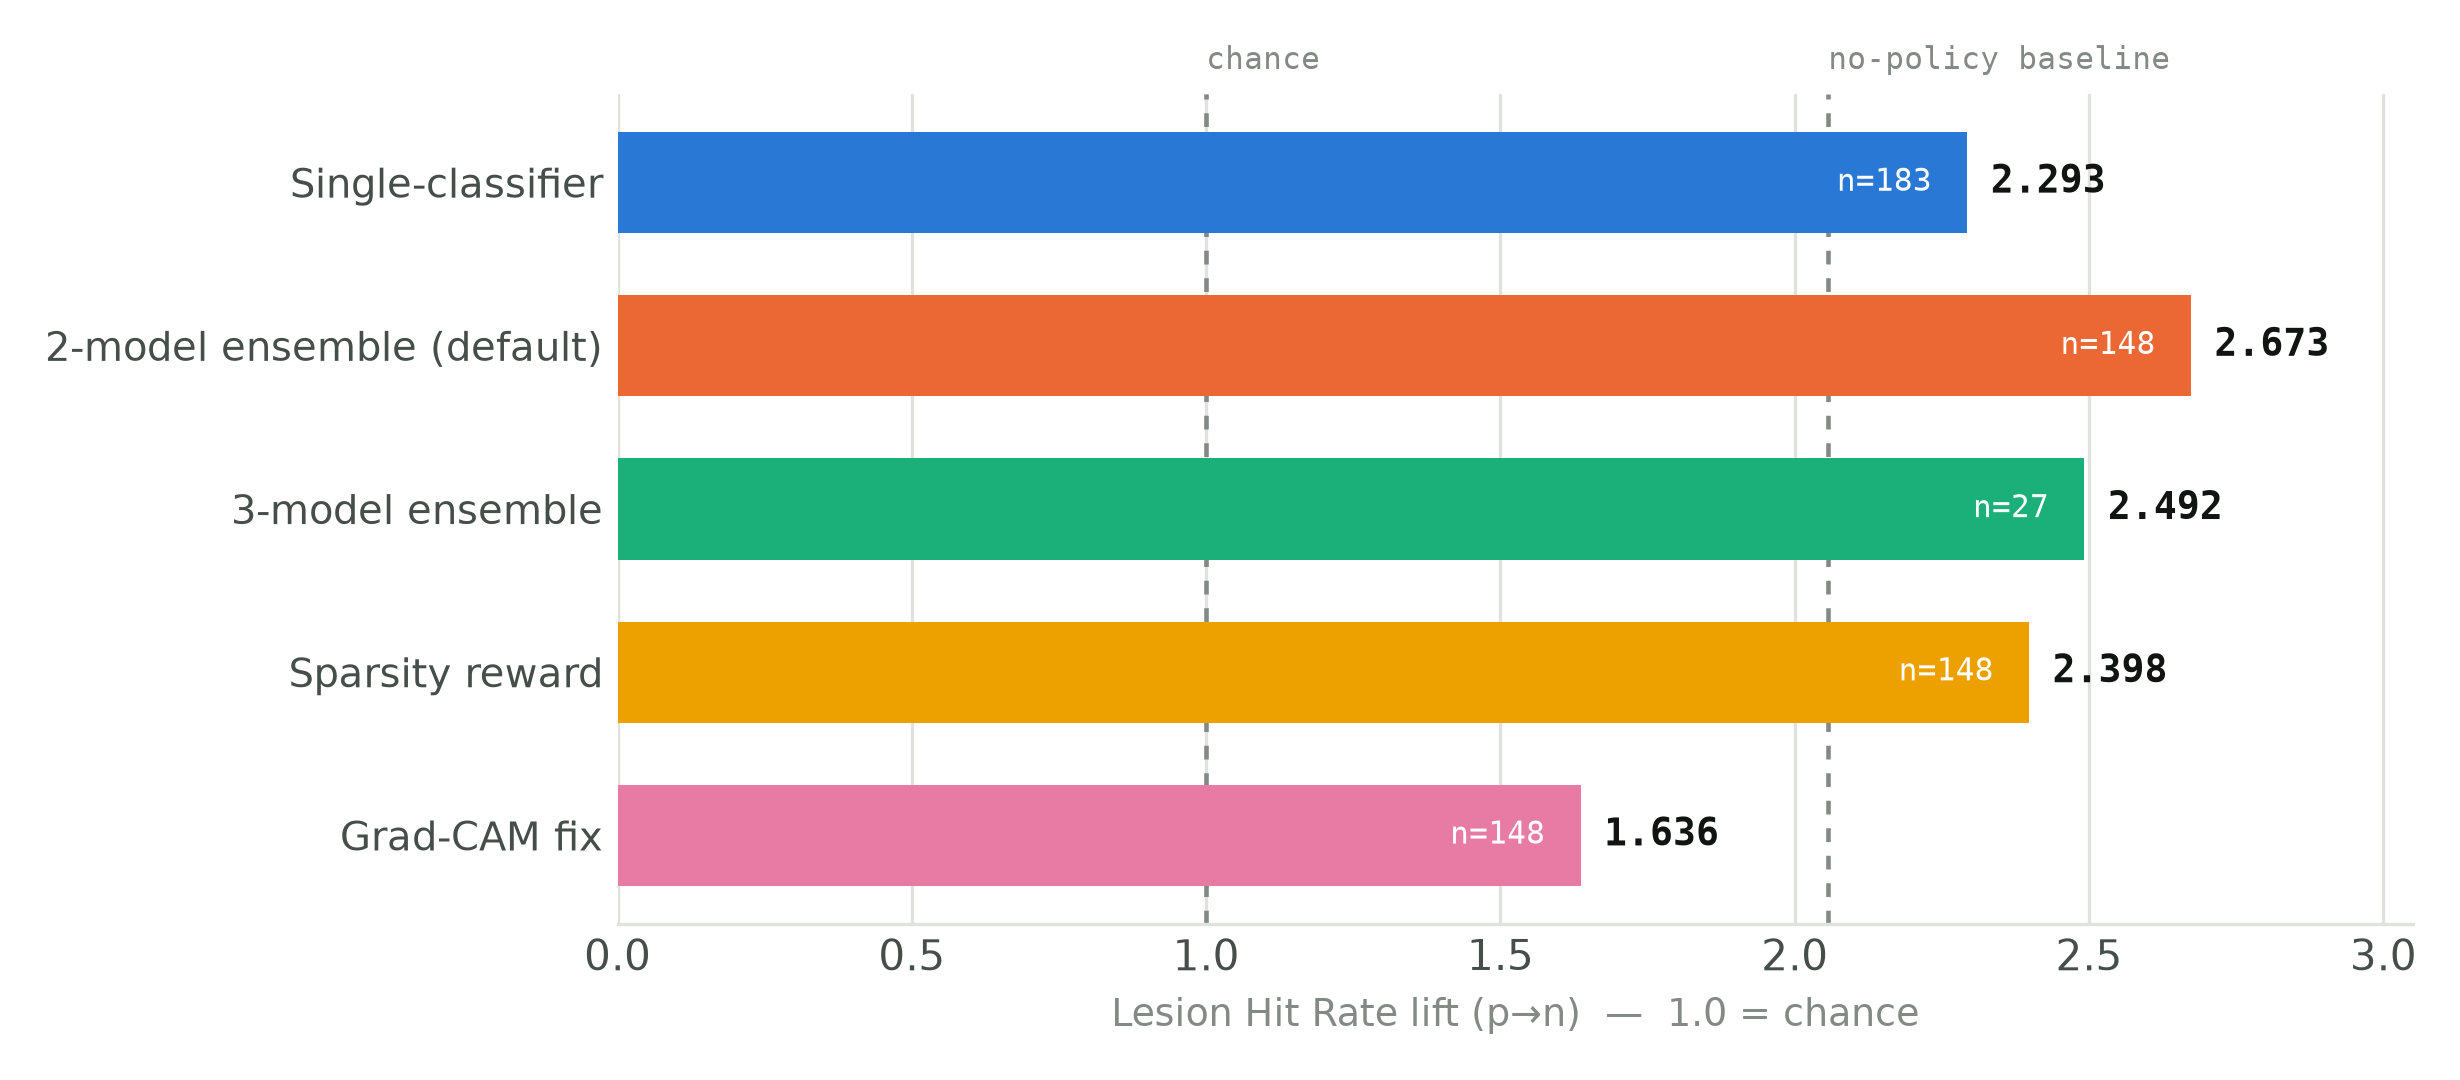
\includegraphics[width=0.9\linewidth]{figures/fig1_lhr_lift.png}
\caption{LHR lift (p$\to$n) across all five trained arms. Dashed lines mark chance (1.0) and the no-policy baseline. The no-policy arm under the same classifier-threshold grouping as the trained arms scores 2.046; the line is drawn at the no-policy value under the label protocol (groups selected by ground-truth label rather than classifier confidence), 2.057, which is indistinguishable at this scale.}
\label{fig:lhr-lift}
\end{figure}

\subsection{Five trained arms}
\label{sec:five-arms}

Every arm in Table~\ref{tab:five-arms} is a policy trained for 800 episodes per direction and evaluated end-to-end, with one training run per arm; none is a cheaper no-policy sweep or an offline proxy. The single-classifier arm predates the split and seeding controls of \S\ref{sec:controls} and was re-scored with corrected code, so its comparisons with the other four arms are not under an identical protocol. LHR verdicts are paired significance tests on the images two arms share, never differences of group means; transfer comparisons use each arm's own bootstrap CI (\S\ref{sec:cv-overstates}).

\paragraph{The ensemble-guided policy beats the single-classifier one, but the comparison is confounded.} Between trained policies, the single-classifier$\to$2-model step rests on a single run per arm: on the 76 shared annotated images the paired LHR-lift test favours the ensemble-guided policy ($d=0.482$, $p=7.1\times10^{-5}$). The two policies differ in more than guidance. The single-classifier policy predates the split and seeding controls, and probably also differs in reward weights, $a_1$ range and background-lock anchoring (\S\ref{sec:controls}; unverified), so this gap cannot be attributed to ensembling alone.
% TODO: single-classifier arm's training config not recorded; differences inferred from development history
Evidence on ensembling itself comes only from a policy-free sweep (three seeds; raw outputs were not preserved): generating without a policy under the label protocol, ensemble guidance raises paired per-image LHR lift over the no-countermeasure baseline by $+0.0694$ ($d=0.221$), $+0.0693$ ($d=0.223$) and $+0.0575$ ($d=0.151$) across three seeds, all with 95\% CIs excluding zero. That effect ($\approx+0.07$) is smaller than the trained comparison and is not a replication of it. Growing the ensemble to three members improves \texttt{pc} n$\to$p transfer from 0.462 to 0.623 with non-overlapping CIs and does not resolve on LHR ($n=12$, paired CI $[-0.298, +0.482]$), so we cannot say whether transfer and lesion targeting dissociate. It also moves \texttt{nih} in the right direction on both counts without separating from noise, and lowers mean CV further to 0.624 (0.685 n$\to$p, 0.563 p$\to$n).

\paragraph{The single-classifier policy beats a random one, but barely.} This comparison is measured against the single-classifier policy ($n=183$ annotated images), not the committed ensemble. Against the random-action arm on the same 183 images: paired lift difference $+0.090$ (95\% CI $[+0.021, +0.160]$), $t=2.551$, $p=0.0116$, Wilcoxon $p=0.0147$, $d=0.189$, trained better on 105/183. The effect is real but small, and considerably smaller than either negative result below.

\subsection{Two negative results}
\label{sec:negative-results}

\paragraph{An annealed sparsity reward fails at its own objective.} Edit concentration has stayed in the 0.21--0.32 band in every arm we measure. The sparsity term was built to address this and had been disabled throughout, leaving its annealing ramp inert. Enabled and isolated against the default, with $\lambda_{\text{sparsity}}$ configured to ramp to its target, concentration moved by less than 0.02 and the n$\to$p fraction of pixels changed went from 0.650 to 0.661. Meanwhile a paired test on the 148 shared annotated images gives a lift gap of $+0.275$ favouring the arm \emph{without} it (95\% CI $[+0.188, +0.363]$, $t=6.229$, $p=4.7\times10^{-9}$, $d=0.512$), and p$\to$n transfer falls from 0.293 to 0.212 with non-overlapping CIs on two of three validators. Without a working spatial mask the term degrades to plain unweighted $L_1$, which discourages edit mass uniformly rather than off-target mass specifically. This is a plausible account of why it competes with precise editing while failing at its own goal.

\paragraph{A Grad-CAM spatial constraint collapses the base task.} In a policy-free sweep (no trained policy), constraining edits to a Grad-CAM~\cite{selvaraju2017gradcam} region lowered LHR lift rather than raising it, so we diagnosed it directly. Scoring 263 member-image observations under the exact ensemble Grad-CAM path used during training contradicted the explanation on record: it is \texttt{chex}, not \texttt{rsna}, that degenerates (66/263, 25.1\% vs.\ 1/263), and it does so concentrated at \emph{low} predicted probability rather than near 0.5, which is consistent with output saturation zeroing the gradient. When \texttt{chex} degenerates the averaged mask falls back toward the least-constrained member alone, and CAM--lesion overlap falls with it (2.052, $n=127$ on clean episodes vs.\ 1.347, $n=23$ on partially degenerate ones). The remedy on record, a finer target layer, does eliminate the degeneracy (0\%/0.4\%) but drops baseline CAM--lesion lift to 1.196, barely above chance.

A policy trained under that remedy moved in the same direction, by a larger margin: CV collapses from 0.838 to 0.017, the paired LHR gap is $+1.037$ favouring the unconstrained arm (95\% CI $[+0.900, +1.178]$, $t=14.660$, $p=1.5\times10^{-30}$, $d=1.205$, better on 141/148 images), and transfer falls across all three validators. This is the largest paired effect size we measure anywhere, and it is against a mechanism introduced specifically to help. Constraining the action space to a finer, less confident CAM region does not trade a degeneracy problem for a localisation problem; it makes the base task substantially harder and every dependent metric degrades with it.

\subsection{Clinical proxy metrics}
\label{sec:clinical-proxies}

% TODO: unverified -- CTR deltas/t/p (n->p, p->n) have no traceable source for committed run
% TODO: unverified -- SCP relative spread 0.19% has no traceable source for committed run
We also computed two clinical proxies under the committed configuration, the Cardio-Thoracic Ratio (CTR) and a costophrenic-recess score (SCP), each with a paired $t$-test on the real-to-counterfactual delta (full results in Supp.~Sec.~E2). CTR shifts by less than 0.01 in both directions, far below the metric's clinical resolution, consistent with a cardiac silhouette that lies largely outside the lung mask gating the edits. SCP is numerically degenerate in this configuration (relative spread 0.19\%), so neither proxy supports a clinical claim.

\subsection{Qualitative examples}
\label{sec:qualitative}

\begin{figure}[H]
\centering
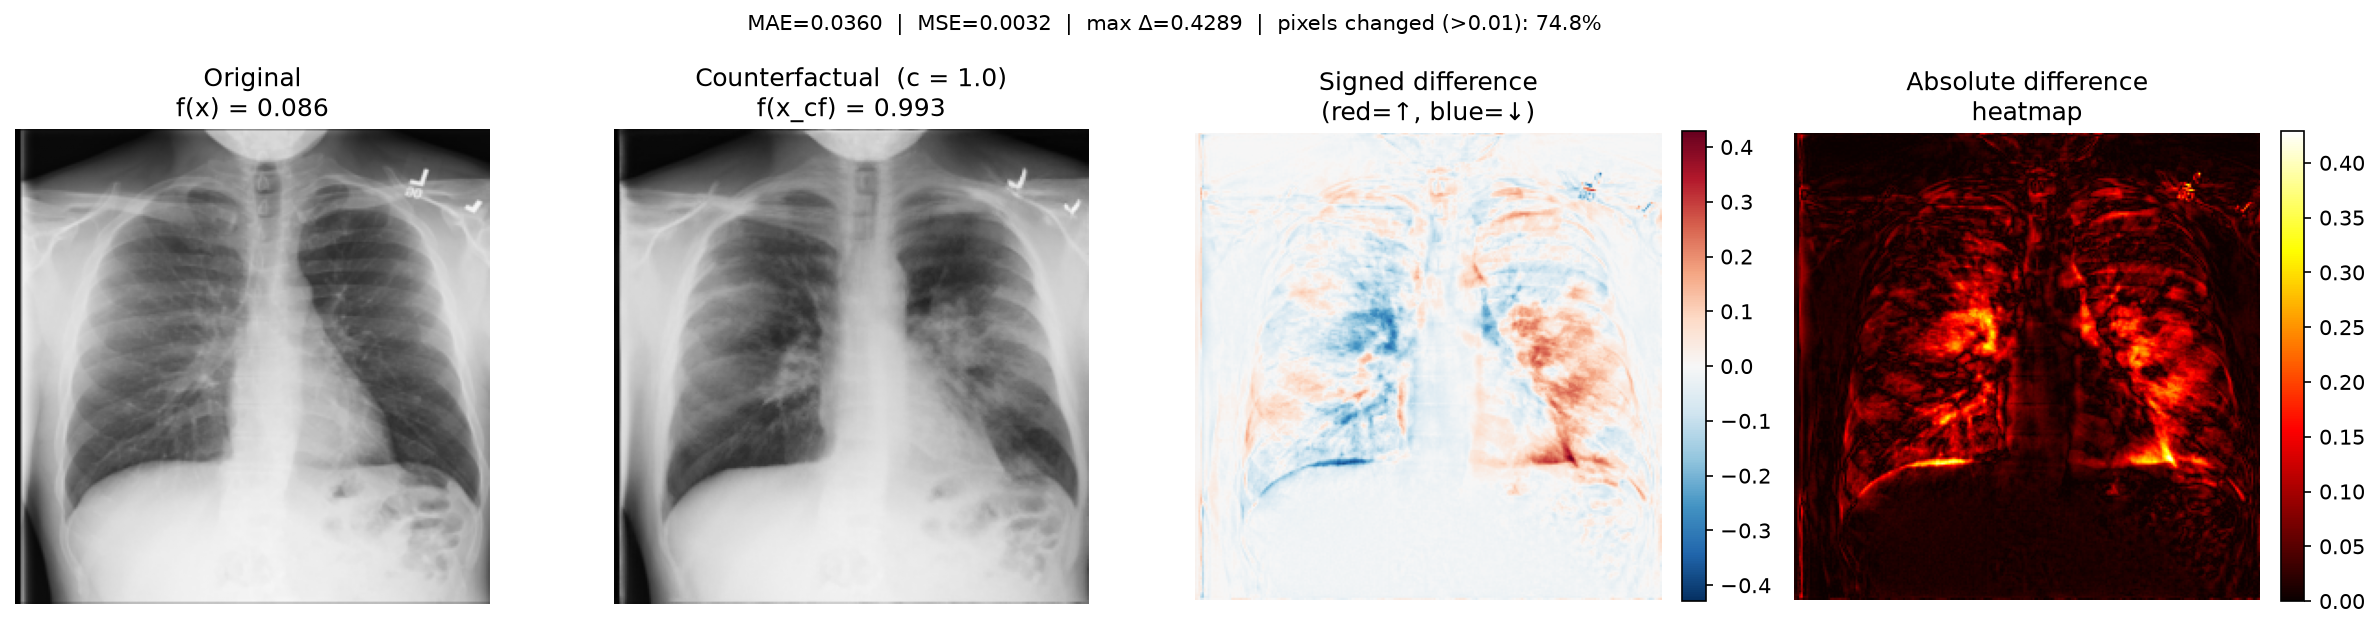
\includegraphics[width=0.9\linewidth]{figures/fig2_qualitative_np.png}
\caption{n$\to$p. Original, counterfactual, signed difference, absolute difference. Change is concentrated over the lung fields where an opacity is synthesized; anatomy outside the lung mask is largely retained, with smaller residual changes visible in the difference maps.}
\label{fig:qualitative-np}
\end{figure}

\begin{figure}[H]
\centering
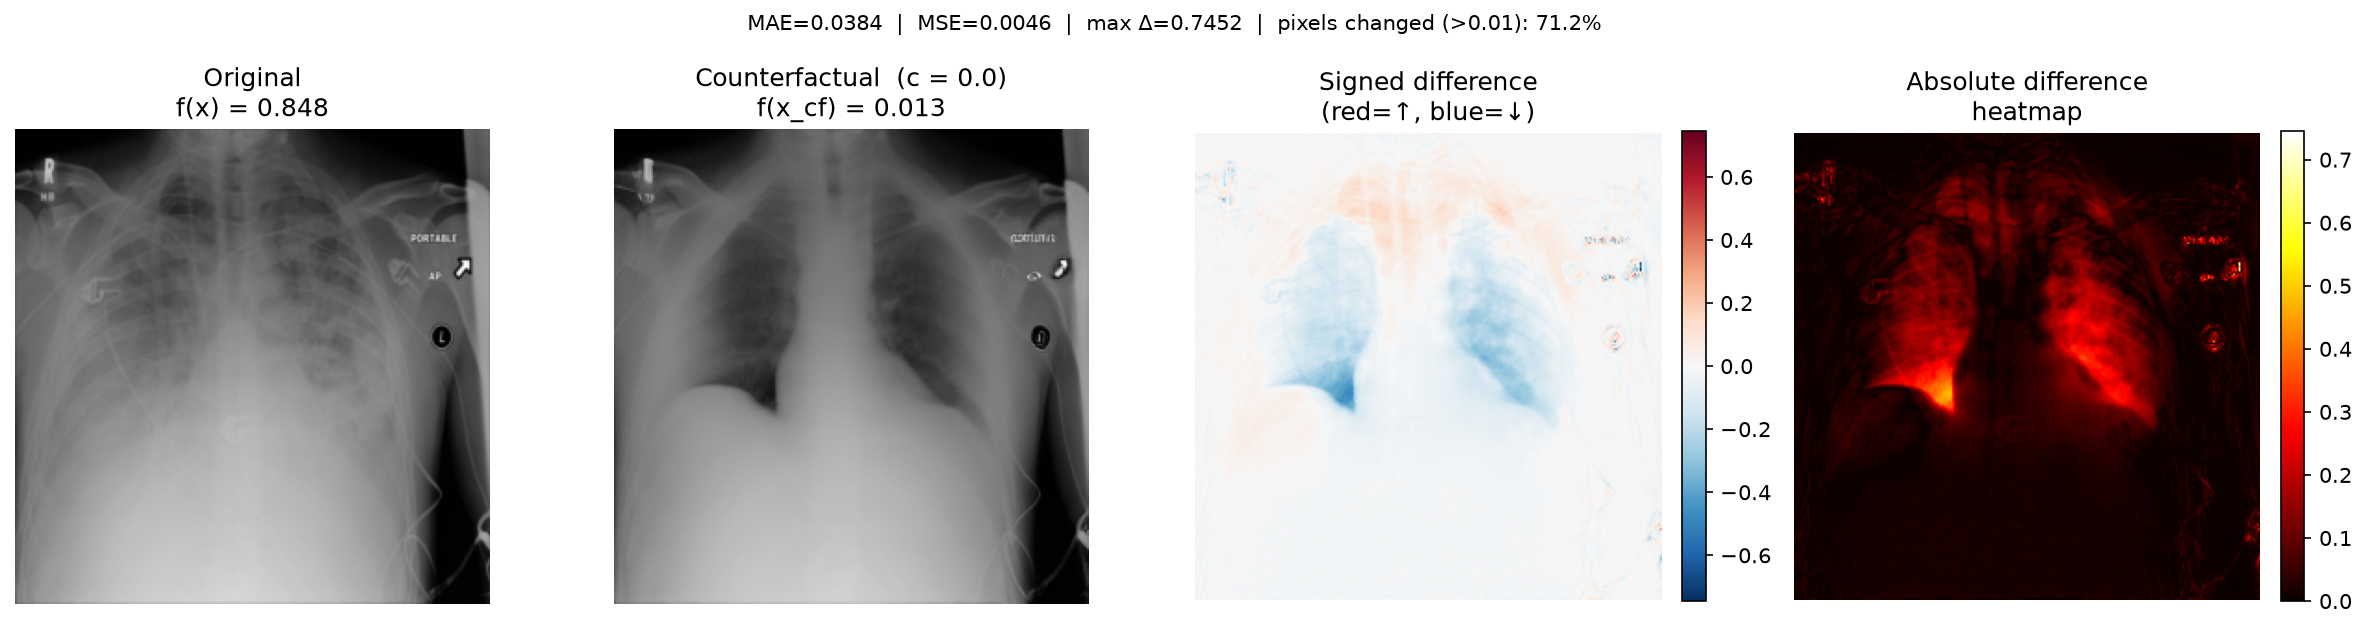
\includegraphics[width=0.9\linewidth]{figures/fig3_qualitative_pn.png}
\caption{p$\to$n. Original, counterfactual, signed difference, absolute difference. Change concentrates bilaterally over both lung fields, consistent with opacity removal, while gross anatomy and external hardware outside the lung mask remain visible, with smaller residual changes (including at the hardware) in the difference maps, consistent with a soft rather than exact lock.}
\label{fig:qualitative-pn}
\end{figure}

Figures~\ref{fig:qualitative-np} and~\ref{fig:qualitative-pn} show counterfactuals from the committed configuration, generated with each policy's mean action. In both, the guidance-classifier score crosses the CV margin ($f(x)=0.086 \to f(x_c)=0.993$ for n$\to$p; $0.848 \to 0.013$ for p$\to$n) while rib cage, mediastinal silhouette and external hardware remain visible outside the edited region; the difference maps still show smaller changes outside the lungs, including at the hardware, as expected from a soft lock. The p$\to$n edit is more concentrated than the n$\to$p one, but both remain diffuse relative to a lesion-shaped edit (\S\ref{sec:main-results}).

\section{Limitations}
\label{sec:limitations}

\begin{itemize}
    \item \textbf{Edits remain diffuse.} No arm we trained moved edit concentration meaningfully; every one sits in the same 0.21--0.32 band regardless of what changed underneath it. Whether diffuseness is fixable at all within a gradient-guidance approach is open.
    \item \textbf{n$\to$p stays adversarial.} On the most independent validator, both policies sit confidently below the 0.15 threshold. The ensemble-guided policy is the better of the two, but that comparison is a single run per arm (below); we cannot show the gap closes. The 0.15 threshold itself is not formally calibrated (\S\ref{sec:cv-overstates} reports counts from 0.10 to 0.25).
    \item \textbf{FOP is not computable offline}, so IP measures a related but not identical property, and SCP is a coarse proxy rather than a trained detector; in the committed configuration it is degenerate rather than merely coarse (\S\ref{sec:clinical-proxies}).
    \item \textbf{Sample size limits several verdicts}, including the 3-model ensemble's p$\to$n results ($n=32$, 27 annotated) and LHR comparison ($n=12$ shared annotated images) and FID, whose variance at $n \sim 200$ in a 1024-d feature space is high.
    \item \textbf{One training run per arm.} The single-classifier and ensemble runs share split, seeds, reward weights, action ranges and anchoring (configuration identical except the guidance flag), but differ in guidance, in classifier-selected groups (78 of 200 p$\to$n sources shared) and in hardware, and no trained-arm gap has a run-to-run error bar. In the single-classifier, 3-model and sparsity arms, the p$\to$n policy is evaluated with the n$\to$p generator adapter rather than the one it was trained with, whereas the committed arm uses its own (\S\ref{sec:directional-policies}), so their paired comparisons against the default also differ in adapter; the Grad-CAM arm's n$\to$p policy was trained for updates 1 to 49 under a different adapter from the one used at evaluation. Re-running the identical protocol on different hardware regenerates different images, so aggregate metrics move by small amounts. % TODO(noise)
Generator fine-tuning, PPO rollouts and the validity probe use only the 80\% training fold, and every evaluated image is in the 20\% test fold. The guidance classifiers and the FID extractor are pretrained models, and the \texttt{rsna} classifier was developed on RSNA data, so we cannot rule out that they have seen evaluation images.
    \item \textbf{The learned schedule is close to fixed.} The committed n$\to$p policy holds its guidance-bias control at 1.298 of 1.30 with three passes per step, and episodes last one to two steps on average, so its behaviour is close to a fixed, aggressive one-shot schedule (training-time diagnostics on 20 sampled episodes; evaluation-time action statistics are not reported). The trained-vs-random comparison ($d = 0.189$, p$\to$n only, $n = 183$) covers only the single-classifier policy, and no comparison against a tuned fixed schedule is available, so the contribution of the learned schedule itself is not isolated. The 37.9M-parameter policy network was trained on at most $800 \times 25 = 20{,}000$ transitions per direction, far fewer given the short episodes, so it may be heavily over-parameterized for this budget. % TODO(J6)
    \item \textbf{Two independent policies} rather than one target-conditioned policy; the harder direction cannot borrow capacity from the easier one.
\end{itemize}

\section{Conclusion}
\label{sec:conclusion}

We presented a PPO-scheduled, LoRA-adapted latent diffusion pipeline for visual counterfactual explanation on chest radiographs, with a soft background lock that largely confines edits to a dilated lung region. We evaluated it under a protocol that pairs the field's conventional classifier-scored validity with a lesion-annotation-anchored hit rate and a held-out transfer ratio. The system attains a 2.60$\times$ lesion-targeting lift over chance, and its ensemble-guided policy improves both lesion targeting and mean held-out transfer over a single-classifier policy whose configuration differs only in the guidance classifier, in a comparison of one training run per arm on partly different evaluation images. It also shows, on its own outputs, that high CV coexists with diffuse edits and adversarial-regime transfer on the most independent validator. Two mechanisms designed to concentrate edits were trained and measured rather than assumed, and both measured as harmful in a single training run each, one by the largest effect size in the study. We take the broader implication to be methodological: CV computed with the guidance classifier should not be reported as a standalone success criterion, and an anchored companion metric (to human annotation, to model independence, or both) costs little and changes the conclusion.

{
    \small
    \bibliographystyle{ieeenat_fullname}
    \bibliography{main}
}


\end{document}
